\section{Technologies}
All the produced code is written in Python (Version 2.7.5). Some of the found research papers use the programming language to create for example a workflow with multiple subtasks. There exists also a plugin for the Amazon Mechanical Turk platform called boto (Version 2.25.0). The API has similar functions as the Java SDK provided by Amazon (Listing \ref{boto_example}). The scikit-learn library (Version 0.13) was used for the machine learning implementation. Therefore, it's possible to create a productive web service with the help of the Django Python web framework in the future.
\lstset{language=Python,caption={boto HIT creation example},label=boto_example}
\begin{lstlisting}
from boto.mturk.connection import MTurkConnection
from boto.mturk.question import QuestionContent,Question,QuestionForm,Overview,...
from boto.mturk.qualification import LocaleRequirement,Qualifications

title = 'Estimate the price of auction items based on title, description and images'
description = ('Take a look at an item description and estimate the corresponding price')
keywords = 'image, pricing, picture, item, estimation'

mtc = MTurkConnection(aws_access_key_id=ACCESS_ID,
                      aws_secret_access_key=SECRET_KEY,
                      host=HOST)
#---------------  BUILD OVERVIEW -------------------
overview = Overview()
overview.append(FormattedContent(html_code))
#---------------  BUILD QUESTION 1 -------------------
qc1 = QuestionContent()
qc1.append_field('Title','Price estimation (USD)')
 
qc1.append(FormattedContent(html_code))
 
fta1 = FreeTextAnswer(None, None, 1)
fta1.constraints.append(NumericConstraint(1, 1000000))          
fta1.constraints.append(RegExConstraint("^\+?([1-9]\d*).\d{0,2}$"))
 
q1 = Question(identifier="price_find",
              content=qc1,
              answer_spec=AnswerSpecification(fta1),
              is_required=True)
#--------------- BUILD THE QUESTION FORM -------------------
question_form = QuestionForm()
question_form.append(overview)
question_form.append(q1)
#--------------- CREATE THE HIT -------------------
qualification = Qualifications()
qualification.add(LocaleRequirement('EqualTo','US'))

hitDetails = mtc.create_hit(questions=question_form,
               max_assignments=5,
               title=title,
               description=description,
               keywords=keywords,
               duration = 60*120,
               reward=0.1,
               qualifications=qualification,
               response_groups = ['Minimal'],
               ) 
\end{lstlisting}
\section{Pure Approach}
The chapter describes the first of two crowdsourcing approaches. The pure one uses only inputs of humans.
\subsection{Ground Truth}
\label{ground_truth}
Real eBay auctions were collected by the API to generate the ground truth for the crowdsourcing experiments. The online auction platform divides their items in eight main categories: Motors, Fashion, Electronics, Collectibles \& Arts, Home \& Garden, Sporting Goods, Toys \& Hobbies and Deals \& Gifts. The ground truth consists of seven items from every category with the exception of the Motor's and Deals \& Gits sections, because the API can't search for items in these categories. First, some keywords were created to touch the desired category: ``Swiss Watch'' (Fashion), ``Smartphone'' (Electronics), ``Football Trading Card'' (Collectibles), ``Coffee Machine'' (Home), ``Soccer shoes'' (Sporting Goods), ``Action Figure'' (Toys) and ``Handbag'' (Fashion). The goal was also to have gender specific and neutral items. An action figure is used by male persons normally, the handbag by females and a smartphone by both. The Finding eBay API provides the method \textit{findCompletedItems} which takes keywords as a parameter and returns a list of completed auction items. The Python script searches for the first sold item which uses US dollar as currency, has a description longer than one-hundred characters and contains of at least three images. Only three images were kept, because most of the auctions present the items with a top, front and side view. Another reason is the clarity for the crowdsourcing tasks. Every ground truth entry has the attributes title, description, category, condition, price and image one to three. The table \ref{basic_ground_truth} (page \pageref{basic_ground_truth}) represents the final ground truth for the further experiments.

\subsection{Tasks Workflow}
The inputs of the pipeline (Figrue \ref{purePipeline}) are images of the item to sell, which were created by the seller. The images from the ground truth are used for the experiments of the thesis. To create item specific information for the auction, four subtasks were designed: 
\begin{itemize}
	\item Generate a title for the auction item
	\item Generate a description of the item
	\item Find one category for the auction item  
	\item Estimate the end price for the auction  
\end{itemize}
The digits in the brackets define the number of assignments. The sellers receive at the end of the pipeline the information which they need to create an auction on eBay. The starting price of the item depends on the sales strategy of the sellers, but the end price should help to find a suitable one. The condition of the item, the auction duration or the payment settings have to be provided by the sellers themselves.
\begin{figure}[h!]
\centering
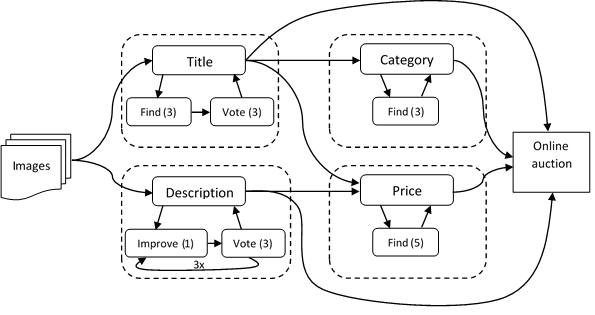
\includegraphics[scale=0.8]{images/pipelines/Pure_Pipeline.png}
\caption{Pure crowdsourcing pipeline}
\label{purePipeline}
\end{figure}

\subsection{Task Design}
At the top of every HIT three images of an auction item are shown. Most of the sellers on eBay present their items with a front, side and top view. Only workers from the United States are allowed to participate in the created tasks, because the ground truth contains only items from there and they have a better feeling for the currency. Some of the tasks need a voting procedure to determine the final answer. The voters have to mandatorily reason their votes to understand the strength of the selected answer. At the end of every task the contributors have the possibility to write down a feedback to the requestor.

Workers who did the same HIT in the past are excluded from the one in the future. This should prevent that they commit the same answer twice. Another restriction is that they can't vote for the own created solution during the voting task. At the beginning of every task, a list of worker IDs is shown and a warning that the answers of them will be rejected. This doesn't avoid the participation of the listed workers by the system, but it works because they won't have a lower approval rate. This solution was easier to implement, but another one has to be used for a productive solution.
\subsubsection{Title}
The goal of this subtask is to generate a clear and concise title for the auction item with at most eighty characters. The auction platform eBay provides some recommendations for a good title. It should contain the item's brand name, artist, or designer. A specification of the item could also be helpful. For example the title could include the size, color, condition, and model number. Correct spelling is a must. All these points will be presented to the workers in the instruction section of the task. To make the instructions clear, an example is also listed:
\begin{table}[h!]
	\begin{center}
	\begin{tabular}{| p{8cm} p{5cm} |}
		\hline
		& \\
		Title: Sony Playstation 4 (black), 1 Controller, New & 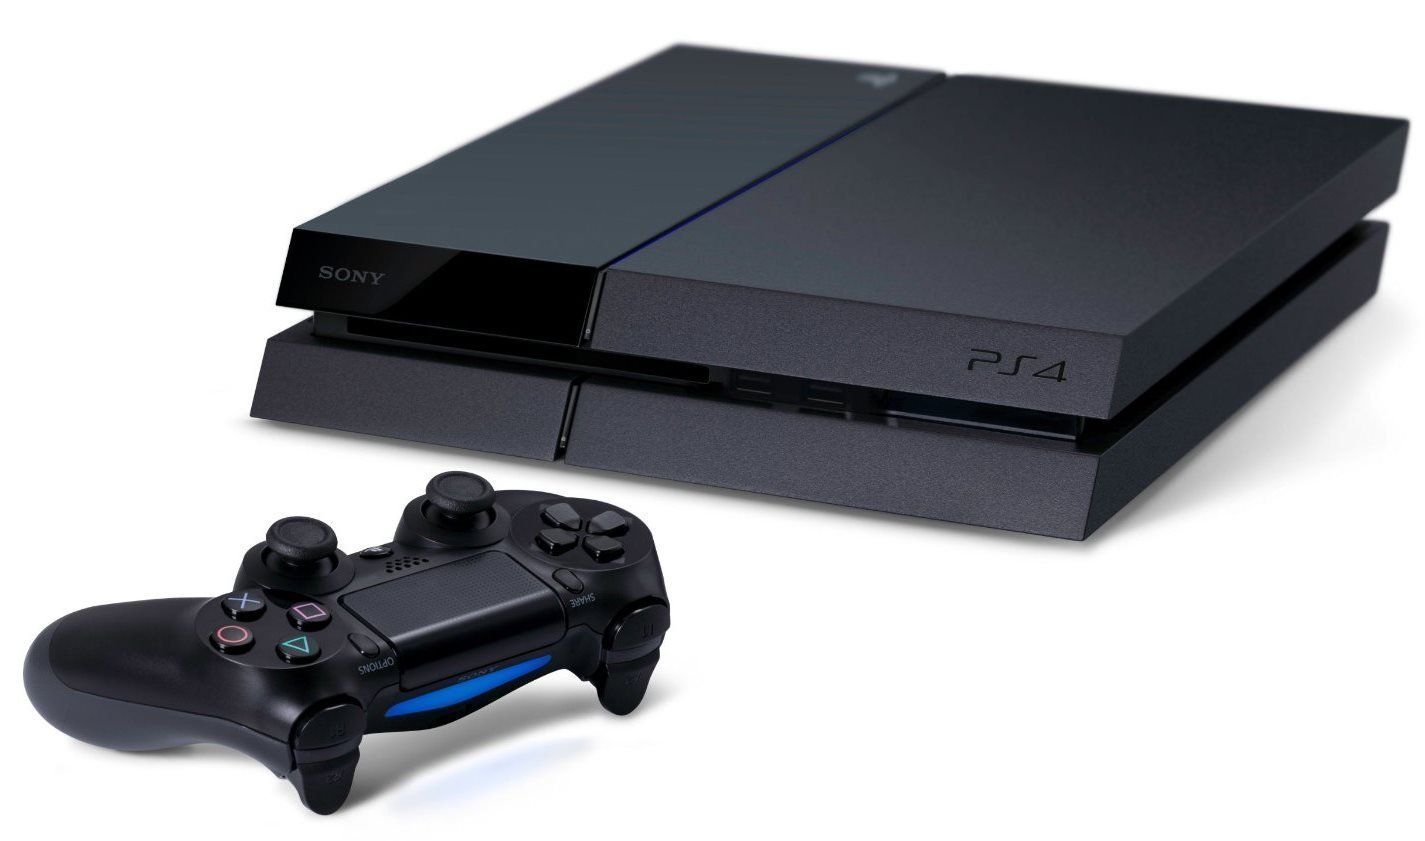
\includegraphics[scale=0.1]{images/ps4} \\
		\hline
	\end{tabular}
	\end{center}
\end{table}
After three titles were created by the crowd, the final title will be elected. If no title receive enough votes, the requester will act as an expert. The expert uses the search engine of the auction platform and decide which title shows more similar items. The turkers will receive \$0.05 for finding a title and \$0.02 for voting.
\subsubsection{Description}
This subtask is a bit different then the others. An iterative task design is used (Subsection \ref{iterative}). First, a worker creates an initial description of the item. Then, the second worker can improve the initial solution or create a new one. Then, the crowd decide which description should be kept and which one should be discarded. One iteration includes an improvement and a voting task. Three iterations were used to generate the description of the auction item. The workers should write approximately five sentences and include specific information like size, color, shape, age, manufacture date, company/author/artist, and notable features or markings. TurKit is a Java application to manage iterative approaches. For an improvement of the text a reward of \$0.2 will be paid, \$0.01 for every participant of the voting procedure.
\subsubsection{Category}
Based on the provided title, the workers have to find the most suitable eBay category for the auction item. The eBay search engine returns one or many categories for a given title. Then the worker has to decide which one matches best. For making a contribution, the workers achieve a payment of \$0.05.
\subsubsection{Price Estimation}
The workers have to guess the end price of the online auction item in US dollar. Reasons for the estimation have to be mentioned additionally. The generated title and description are available for a better understanding of the picture contents. The workers have the possibility to list missing information for a more precise estimation. The participants receive a gratification of \$0.05.

\subsection{Variations}
The prior section describes the standard composition of the tasks. To survey the behaviour of the workers, some design modifications were made: 
\subsubsection{Image Quantity and Quality}

All available images were presented to the crowd with the highest image resolution. The basis setting of the tasks shows only the first three images. The table \ref{tab:res_img} illustrates the number of additional images per item and the corresponding resolutions.
\begin{table}[h!]
	\begin{center}
	\begin{tabular}{| p{4.33cm} | p{4.33cm} | p{4.33cm} |}
		\hline
		\textbf{Ground Truth ID} & \textbf{Total Images} & \textbf{High Resolution (1600 x 1200)} \\
		\hline
		1 & 6 & Yes \\
		\hline
		2 & 3 & No \\
		\hline
		3 & 4 & Yes \\
		\hline
		4 & 7 & No \\
		\hline
		5 & 9 & Yes \\
		\hline
		6 & 3 & Yes \\
		\hline
		7 & 4 & Yes \\
		\hline
	\end{tabular}
	\end{center}
	\caption{Ground truth image quantity/quality}
	\label{tab:res_img}
\end{table}
\subsubsection{Market Price}
The actual market price of the items (Table \ref{tab:market_prices}) was mentioned in the price estimation task. The web service pricegrabber.com was used to find reliable and consistent prices. 
\begin{table}[h!]
	\begin{center}
	\begin{tabular}{| p{6.5cm} | p{6.5cm} |}
		\hline
		\textbf{Ground Truth ID} & \textbf{Price (in USD)} \\
		\hline
		1 & 69.00 \\
		\hline
		2 & 399.99 \\
		\hline
		3 & 49.99 \\
		\hline
		4 & 299.00 \\
		\hline
		5 & 189.99 \\
		\hline
		6 & 44.99 \\
		\hline
		7 & 289.99 \\
		\hline
	\end{tabular}
	\end{center}
	\caption{Ground truth market price}
	\label{tab:market_prices}
\end{table}
\subsubsection{Commission}
This section describes the idea of an additional incentive for the workers which is added to the reward of MTurk tasks as a bonus. If an auction item will be sold successfully on eBay then all contributors of the crowdsourced result will receive a commission of the end price. The ground truth contains already completed eBay auctions and therefore the criterion of the bonus has to be determined otherwise. Only those created auctions which get more votes, during the evaluation process, than the ground truth will receive a commission. The table \ref{comm_perc} shows the distribution of the percentages. The bonus can be between 2.55\% and 4.9\% of the end price. The range of the end prices in the ground truth goes from \$4.99 (watch) to \$201 (coffee machine). From this it follows that the commission can be between \$0.127 (2.55\% of \$4.99) and \$9.85 (4.9\% of \$201). The differences of the worker behaviour and a potential quality intensification will be investigated. 
\begin{table}[h!]
	\begin{center}
	\begin{tabular}{| p{3.25cm} | p{3.25cm} | p{3.25cm} | p{3.25cm} |}
		\hline
		\textbf{Name of task} & \textbf{Number of assignements (Min)} & \textbf{Number of assignements (Max)} & \textbf{Percentage of commission (in \%)} \\
		\hline
		Title (Finding) & 1 & 1 & 0.25 \\
		\hline
		Title (Voting) & 2 & 3 & 0.1 \\
		\hline
		Description (Improving) & 1 & 1 & 1.0 \\
		\hline
		Description (Voting) & 2 & 2 & 0.05 \\
		\hline
		Category & 2 & 3 & 0.25 \\
		\hline
		Price & 1 & 5 & 0.5 \\
		\hline
		Total (Min) & & & 2.55 \\
		\hline
		Total (Max) & & & 4.9 \\
		\hline
	\end{tabular}
	\end{center}
	\caption{Commission percentages}
	\label{comm_perc}
\end{table}

\subsubsection{Non-branded Item}
All of the ground truth items have visible brand labels. Some are more famous (Apple\footnote{http://www.apple.com}, Puma\footnote{http://www.puma.com}) than the others (Palisades, Powman Sterling). Information about the brands and their manufactured items can be found easily. Describing an unknown object is more difficult. A non-branded item is put into the pipeline to research the ability of the workers to handling such items (Table \ref{nonbranded_ground_truth}, page \pageref{nonbranded_ground_truth}). 

\section{Hybrid Approach}
The second approach is illustrated after this introduction sentence.
\subsection{Ground Truth}
A lot of sold items were collected by the help of the eBay API. The used methods were the same as in the prior ground truth generation (Chapter \ref{ground_truth}). After all the necessary data were collected, the Python script splits the data shuffled into a training and test set. The training set contains about 70 percent of the whole data. All the consecutively steps (Data analysis, feature ranking) will use the training set until the performance of a classifier will be proved on the test set. The continuous target values are also converted into price classes to use classification algorithms later on. The range of the classes depends on the highest price of the item type. The goal was to generate the same number of classes for every category. The ground truth was generated for three different item types:
\begin{table}[h!]
	\begin{center}
	\begin{tabular}{| p{2.6cm} | p{2.6cm} | p{2.6cm} | p{2.6cm} | p{2.6cm} |}
		\hline
		\textbf{Item type} & \textbf{Total number of auctions} & \textbf{Size of training set} & \textbf{Size of test set} & \textbf{Price class range (USD)} \\
		\hline
		Apple iPhone & 2'299 & 1'609 & 690 & 25 \\
		\hline
		Hot Wheels Cars, 1:64, Ford Mustang & 945 & 661 & 284 & 2 \\
		\hline
		Sony Playstation & 943 & 660 & 283 & 25 \\
		\hline
	\end{tabular}
	\end{center}
	\caption{Ground truth sets for machine learning}
\end{table}
\subsection{Tasks Workflow}
The hybrid pipeline (Figure \ref{hybridPipeline}) works same as the pure one except that two subtasks are supported by machines.
\begin{figure}[h!]
\centering
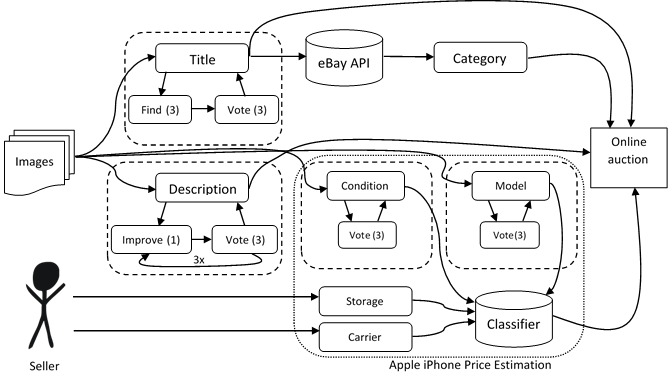
\includegraphics[scale=0.8]{images/pipelines/Hybrid_Pipeline.png}
\caption{Hybrid crowdsourcing pipeline}
\label{hybridPipeline}
\end{figure}
\subsection{Task Design}
The design of the tasks is similar to the pure approach except of the two subtasks category and price.
\subsubsection{Category}
The implementation finds the most suitable category by using the eBay Finding API based on the output of the title task. Most of the titles are too specific and the API doesn't return a category. The algorithm reduces the number of words until a category is found. The used method returns a sorted histogram of categories.
\subsubsection{Price Estimation}
The goal of the task is to estimate the end price of the auction by using a machine learning approach. The input features are built by a combination of crowdsourced and user specified information. The pipeline shows the required fields to estimate the price of an iPhone. The model and the condition of the item is determined by the crowd. The seller provides the information which aren't possible to collect by others. The storage size of the phone which isn't visible, for example. If all needed features are available then the machine learning algorithm will produce an end price.
\subsection{Pre-processing}
During the collection of the sold items some pre-processing steps were necessary to produce accurate results by the machine learning algorithms. All the recorded features were normalised within the parameters of 0 and 1 to generate a uniform feature space. The target labels (price) remain unaffected. 
Another problem was the quantity of items for a single auction. The quantity field of the entry was one, but the auction contains a lot or a set of items. If an auction title contains a certain keyword (``Set'', ``Lot'', ``Pack'' or ``Bundle'') then the entry will be ignored.
\subsection{Feature Extraction}
The extracted features are divided into three categories.
\subsubsection{Item Specific Features}
The features of this subsection are dependent of the present item category. The number of features is reliant on the available item specific fields provided by the eBay system.
\paragraph{Apple iPhone}
The iPhone made by Apple is available in eight models. The first generation was released in 2007, the last model 5S in 2013. Every model comes with different storage sizes (from 8GB to 64GB). The values for the condition property on eBay depend on the corresponding item category. All the values are nominal and will be converted to numerical.
\begin{table}[h!]
	\begin{center}
	\begin{tabular}{| p{2.6cm} | p{2.6cm} | p{2.6cm} | p{2.6cm} | p{2.6cm} |}
		\hline
		\textbf{Name} & \textbf{Description} & \textbf{Values} & \textbf{Range} & \textbf{Data type} \\
		\hline
		Model & The model of the iPhone where 0 is the oldest generation and 7 the newest & 1st, 3G, 3GS, 4, 4S, 5, 5C, 5S & [0, 7] & Integer \\
		\hline
		Storage & The size of the storage of the smartphone & 8GB, 16GB, 32GB, 64GB & [1, 4] & Integer \\
		\hline
		Condition & The condition of the iPhone & New, New other, Manufacturer refurbished, Seller refurbished, Used, For parts or not working & [1, 6] & Integer \\
		\hline
	\end{tabular}
	\end{center}
	\caption{iPhone specific features}
\end{table}

\paragraph{Mattel Hot Wheels Cars}
Mattel\footnote{http://www.mattel.com} produces diecast car models in different sizes and series. Cars with a ratio of 1:64 are the most popular ones. The collected data contains only Ford Mustang cars, because they are very famous in the US and it should be possible to distinguish between different models. The exact model is indicated by a date.
\begin{table}[h!]
	\begin{center}
	\begin{tabular}{| p{2.6cm} | p{2.6cm} | p{2.6cm} | p{2.6cm} | p{2.6cm} |}
		\hline
		\textbf{Name} & \textbf{Description} & \textbf{Values} & \textbf{Range} & \textbf{Data type} \\
		\hline
		Model & The model of the Ford Mustang where 1964 is the oldest and 2014 the newest & & [1964, 2014] & Integer \\
		\hline
		Condition & The condition of the car & New, Used & \{1, 2\} & Integer \\
		\hline
	\end{tabular}
	\end{center}
	\caption{Hot Wheels specific features}
\end{table}

\paragraph{Sony Playstation}
Sony's\footnote{http://www.sony.com} Playstation exists in ten versions. Two of them are portable and for the second and third model of the console is a slim version available. Every device has a region code or all data carriers are readable. There is no simple way to extract the storage size of the consoles at the moment, because eBay doesn't provide a field for this specific information.
\begin{table}[h!]
	\begin{center}
	\begin{tabular}{| p{2.6cm} | p{2.6cm} | p{2.6cm} | p{2.6cm} | p{2.6cm} |}
		\hline
		\textbf{Name} & \textbf{Description} & \textbf{Values} & \textbf{Range} & \textbf{Data type} \\
		\hline
		Model & The model of the Playstation & 1, 2, 2 Slim, 3, 3 Slim, 4, Vita, Portable & [0, 7] & Integer \\
		\hline
		Region Code & The region code of the console & Not specified, NTSC, PAL, Region free & [0, 3] & Integer \\
		\hline
		Condition & The condition of the item & New, New other, Manufacturer refurbished, Seller refurbished, Used, For parts or not working & [1, 6] & Integer \\
		\hline
	\end{tabular}
	\end{center}
	\caption{Playstation specific features}
\end{table}

\subsubsection{Auction Specific Features}
The auction itself is described by the features in this section. The list (Table \ref{tab:auction_features}) contains some timing and shipping information. Also the number of pictures and the description length could have an influence to the result of the auction. All values are numerical.
\begin{table}[h!]
	\begin{center}
	\begin{tabular}{| p{2.6cm} | p{2.6cm} | p{2.6cm} | p{2.6cm} | p{2.6cm} |}
		\hline
		\textbf{Name} & \textbf{Description} &  \textbf{Range} & \textbf{Data type} \\
		\hline
		Duration & The duration of the auction in days & \{1, 2, 3, 7, 10\} & Integer \\
		\hline
		Number of pictures & Number of pictures attached to the auction & [1, 12] & Integer \\
		\hline
		Length of description & Length of the item description & [0, 500'000] & Integer \\
		\hline
		End weekday & The last weekday of the auction duration & [1, 7] & Integer \\
		\hline
		Start weekday & The weekday of the creation date & [1, 7] & Integer \\
		\hline
		End hour & At what hour the auction was ended & [0, 23] & Integer \\
		\hline
		Global shipping & The item will be shipped over the whole world or not & \{0, 1\} & Boolean \\
		\hline
		Shipping locations & The number of countries where the item will be shipped & [0, 249] & Integer \\
		\hline
		Shipping type & Specifies the calculation of the shipping costs & [0, 7] & Integer \\
		\hline
		Returns accepted & If the buyer can return the item or not & \{0, 1\} & Boolean \\
		\hline
		Handling time & How many days will it take until the item is put in the mail once the seller receive payment & \{1, 2, 3, 4, 5, 10, 15, 20\} & Integer \\
		\hline
	\end{tabular}
	\end{center}
	\caption{Auction specific features}
	\label{tab:auction_features}
\end{table}
\subsubsection{Seller Specific Features}
These features (Table \ref{tab:seller_features}) characterise the seller who created the auction. Every user on eBay has the possibility to give a positive, neutral or negative feedback after every transaction. The rating system awards stars with twelve different colors for trustful sellers. After ten positive feedbacks the user receives a yellow star for example. Therefore, the nominal value has to be converted to an integer.
\begin{table}[h!]
	\begin{center}
	\begin{tabular}{| p{2.6cm} | p{2.6cm} | p{2.6cm} | p{2.6cm} | p{2.6cm} |}
		\hline
		\textbf{Name} & \textbf{Description} &  \textbf{Range} & \textbf{Data type} \\
		\hline
		Seller rating & Percentage of positive feedbacks & [0, 100] & Float \\
		\hline
		Seller rating count & Number of positive minus negative buyer feedbacks & [0, 12] & Integer \\
		\hline
	\end{tabular}
	\end{center}
	\caption{Seller specific features}
	\label{tab:seller_features}
\end{table}
\subsection{Data Analysis}
This chapter takes a closer look at the collected data. Every item category has an attribute model. The price of the smartphones depends on the date of appearance (Figure \ref{model_price_iphone}). The newest iPhone 5S produces the highest price, the second generation the lowest one. The debut feature produced by Apple has a high value for collectors and are traded higher than some later versions. The mean values of every iPhone model can be roughly estimated by a quadratic function. The data of the Playstation shows similar characteristics for the average prices related to the price feature. The Hot Wheels Cars have a completely different price distribution. There is no visible pattern for the recorded models. The Ford Mustang from 1983 has the highest average price of \$27.02, but was sold only once. The rarity of the items has a higher influence to this category than to the other ones.

The histogram of the iPhone (Figure \ref{model_hist_iphone}) illustrates that the model 4 and 4S are involved in about 60\% of the collected auctions. The Playstation 3 Slim is the most dominate console (about 39\%). The previous model of the actual one is dominating the online marketplaces. The 1967 and 1971 are the most popular Mustang models in the data set with 31 different types.

An executed feature ranking \cite{guyon} with SVMs indicated surprisingly that some features aren't as important as expected. The model of a car has only a small influence to the end price. The condition of the item and the duration of the auction are important for all the three tested categories.
\begin{figure}
\centering
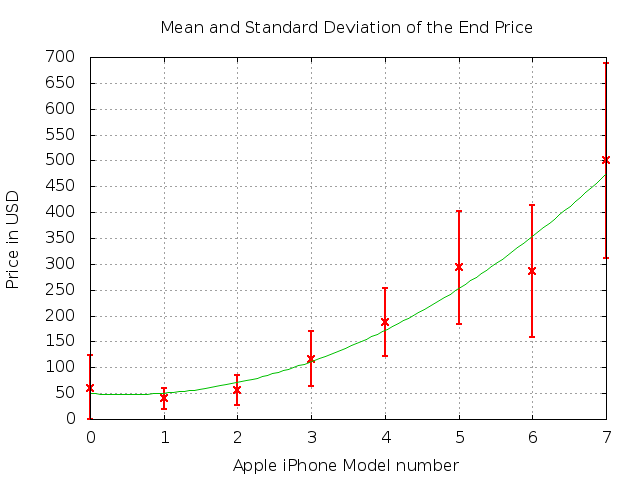
\includegraphics[scale=0.5]{images/plots/iphone/price_model_iphone.png}
\caption{Model/Price scatter plot (iPhone)}
\label{model_price_iphone}
\end{figure}
\begin{figure}
\centering
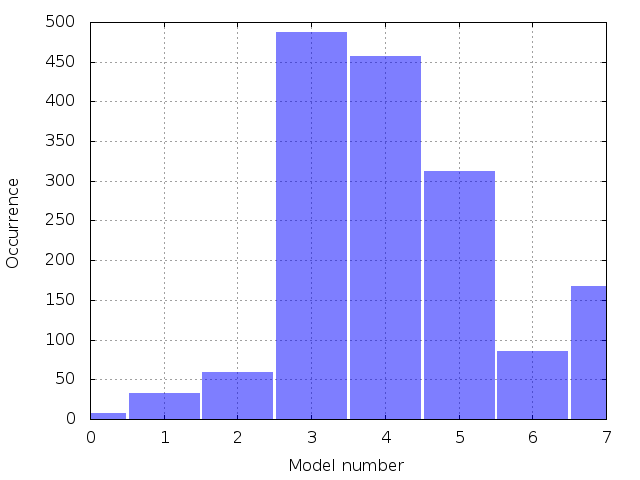
\includegraphics[scale=0.5]{images/plots/iphone/hist_model_iphone.png}
\caption{Model histogram (iPhone)}
\label{model_hist_iphone}
\end{figure}
\subsection{Machine Learning Algorithms}
Three machine learning algorithms were used to estimate the price. The theoretic knowledge about the algorithms is given in the following of this preface.
\subsubsection{k-Nearest Neighbours}
The kNN algorithm \cite{knn} represents every sample of the training set in an \textit{n}-dimensional feature space where \textit{n} are the total number of features. The class correspondence of the data points is stored too. For the classification of a test sample, the \textit{k}-nearest neighbour data points are determined. Usually, the Euclidian distance is used to calculate the distance between the points in the \textit{n}-dimensional space. The data point is assigned to the class with the majority in the neighbourhood. If no class is dominant then the \textit{k} is decreased by one until the tie is broken. The standard configuration of the algorithm uses uniform weights for the data points. This means that each point in the neighbourhood has the same influence to the result. Another way to determine the weight of a neighbour is to calculate the inverse of the distance to the point under supervision. The algorithm can also be used for continuous values (Regression). In that case, the average value of the \textit{k}-neighbours will form the regression output.

Seller of online auction items compare previous auctions for the same or similar ones to estimate the price. The kNN algorithm works similar and should provide good results. 
\subsubsection{Multiclass Support Vector Machines}
Normally, Support Vector Machines (SVMs)\cite{svc} are used for binary decisions. To classify multiple classes, the ``one-versus-one'' approach is used. If there exists three classes in total, three SVMs (Class A vs. class B, class A vs. class C, class B vs. class C) are needed. The class with the majority of the votes will be the resulting output. The idea of the classifier is to map the inputs into a high-dimensional feature space for an accurate separation by one or more hyperplanes. The hyperplanes can be linear or non-linear (e.g. Polynomial, Gaussian). The margin between the two classes should be maximised, points on the margin are called support vectors. These vectors have a higher influence to the classification. The class membership of an input sample is determined by the location (relating to the margin) of the point in the high-dimensional feature space. A regression based implementation of the algorithm is available as well\cite{svr}.

Some online auctions for the same item produce a higher price of sale than others (outliers). The goal is that such observations have no or only a small influence to the price prediction. SVMs use a subset of points (Support vectors) to determine the class membership. Other points which are far away from the margin have no influence to the final result and the auction outliers should play this role. Therefore, the SVMs could be a good solution for the discussed problem. 
\subsubsection{Random Forest Classifier}
The Random Forest classifier was introduced by Leo Breiman in 2001\cite{breiman}. The classifier combines multiple randomised decision trees and average their results for a final decision. The size of the forest is one of the parameters of the classifier, the number of features considered for a split node another one. Because all the trees are considered, the calculations of the outputs can be parallelised. The paper explains the creation of the trees, the training procedure and gives the mathematical background to understand all the information.

The price of an item is mostly dependent on the number of features and the quality or quantity of them. If a certain feature is available then the seller expect that the end price of the auction will be higher than without this feature. For example, the car with an integrated air conditioning will be sold for a higher price than the same one without the air conditioning. Therefore, a decision tree should help to create a decision process based on the available features which seems like a natural human behaviour. One tree alone is not enough to cover all the different circumstances. 
\subsection{Parameter Search}
To find the best parameters of the introduced machine learning algorithms, a grid parameter search was done. The idea of this approach is to train a given classifier to predefined sets of values and keep the ones with the best performance. A 5-fold cross-validation was used to generate separate training and test sets. The original test set stays untouched. The method splits the set into five equally sized subsets. Four subsets are used for training and one for testing, then the roles change clockwise until every subsets was used as test set. The final result is calculated by the average performance of every iteration. The procedure helps to avoid overfitting of the models.
\subsection{Signifigance Tests}
The significance test should help to find out if the results of two classifiers are happened by chance. First, the null hypothesis H$_{0}$ has to be formulated:\\\\
``The mean performance of classifier A is the same as classifier B''\\\\
The hypothesis can be rejected if the calculated \textit{p}-Value is lower than 5\%. The results of the classifiers are not normally distributed, therefore the following tests were used. 
\subsubsection{G-Test}
The G-Test\cite{gtest} is used for the nominal labels and is appropriate for multiple classes. It is a modification of the Chi-Squared test, but can handle smaller observed frequencies in a cell of the contingency table. Because not every price class occurs in the outputs of the classifiers, the G-Test is favoured over the Chi-Squared test. The results of two classifiers are grouped into a 2 x \textit{N} contingency table where the rows represent classifier A and B. \textit{N} is the total number of different classes in both results. The outputs of the algorithms A and B are recorded at every cell in the table. After that, the expected frequency is calculated for every cell. Based on these two tables the G-Test algorithm calculates the corresponding \textit{p}-Value. 
\subsubsection{Wilcoxon-Signed-Rank Test}
The Wilcoxon-Signed-Rank test\cite{wilcoxon} is an alternative to the paired t-test, but assumes that the population is not normally distributed. The test verifies if the difference between the two given outputs of the regression algorithms is symmetric about zero. First, the absolute differences will be sorted in ascending order. Then the samples receive a rank starting with the smallest as 1. Then a \textit{p}-value will be calculated.
